\documentclass[11pt]{article}
\renewcommand{\baselinestretch}{1.5}
\setlength{\oddsidemargin}{0pt}
\setlength{\evensidemargin}{0pt}
\setlength{\topmargin}{-20pt}
\setlength{\headsep}{10pt}
\setlength{\headheight}{14pt}
\addtolength{\textheight}{1.3in}
\setlength{\textwidth}{6.2in}
\usepackage{amsmath}
\usepackage{amsfonts}
\usepackage{enumerate}
\usepackage{hyperref}
\usepackage{tabularx}
\usepackage{makecell}
\usepackage{graphicx}
\usepackage{authblk}
\usepackage{natbib}
\usepackage{caption}
\usepackage{subcaption}
\usepackage{algorithm}
\usepackage{float}
\usepackage{listings}
\usepackage{dsfont}
\usepackage{booktabs}
\usepackage{bm}
\usepackage{algpseudocode}



\title{A Two-Step Anomaly Detection Approach for Spatiotemporal Raster Data with its Application to Wildfire Detection}

\author[1]{Kehui Yao}

\affil[1]{Department of Statistics, University of Wisconsin-Madison}	



\date{}

\begin{document}

\maketitle

\begin{abstract}
Spatiotemporal (ST) raster data, consisting of measurements taken at specific locations and times, are common in fields such as environmental monitoring, climate science, and natural disaster management. Detecting anomalies in these data is crucial for applications such as wildfire monitoring. This chapter develops a novel two-step anomaly detection algorithm for ST raster data, integrating neural network-based and statistical time series anomaly detection methods with a locally adaptive weighting and screening (LAWS) strategy. The algorithm identifies anomalies by first generating p-values for each location-time point and then aggregating them using LAWS to identify spatial anomalies. Extensive simulations demonstrate the method's accuracy and scalability, particularly in large datasets. The algorithm's application to wildfire detection in the Sakha Republic demonstrates its practical effectiveness in identifying affected regions, aiding natural disaster management.

\end{abstract}

\section{Introduction}
Spatiotemporal (ST) raster data are measurements of continuous or discrete ST fields at fixed locations in space and fixed points in time, which are commonly encountered in real-world applications such as environmental monitoring, climate science, agriculture, public health, and disaster management. Examples of ST raster data include measurements collected by ground-based sensors of ST fields like traffic and air quality, as well as satellite images captured at regular revisit times. 
 
 Anomaly detection is widely used in applications such as fraud detection, intrusion detection, and military surveillance. Anomaly detection identifies data points that significantly deviate from the expected patterns in a dataset.  Detecting anomalies in ST raster data is useful in many areas. For example, in wildfire monitoring, we detect areas with unusually high thermal signatures, which could indicate the start or spread of wildfires. In hurricane forecasting, we detect unusual patterns in cloud formation and movement that could signal a hurricane's development or change in direction. In drought and flood prevention, we identify rapidly changing water levels. In disease management, we detect sudden increases in regions with higher-than-usual disease incidences.


In ST raster data, anomalies are typically spatially contiguous groups of locations (regions) that consistently show anomalous values for one or a short duration of time stamps. Most approaches for detecting anomalies in ST raster data decompose the problem by first treating the spatial and temporal properties of outliers independently before merging them in a post-processing step. \citet{paschalidis2008spatio} proposed a method to identify traffic anomalies. They first detect anomalies in individual traffic series and then incorporate spatial information to analyze traffic activities at various network locations. \citet{faghmous2012novel} developed a novel method for ocean eddy anomaly detection by first identifying individual time series with eddy-like behavior, and then checking neighboring time series at each time step. If enough neighbors are candidates at a given time stamp, the group is labeled as an eddy. In contrast, several studies first find anomalous spatial regions and then combine them over time to identify ST anomalies. For instance, \citet{wu2010spatio} used a spatial scan statistic to find the top-k contiguous groups of locations with anomalous precipitation at each time stamp, then combined them over time to identify ST anomalies.





%\section{Time Series Anomaly Detection}\label{sec: time series anomaly detection}
Time series data often show smooth changes or follow predictable patterns. In time series, anomalies are usually defined as two types. The first type is point anomaly: an individual data point in a time series significantly differs from the rest. The second type is collective anomaly: a group of consecutive data points significantly deviate from the normal behavior or pattern of the data, even if the individual data points are not extreme on their own. 

Many statistical methods in the time-series anomaly detection literature involve fitting a model to the time series data and examining residuals (the differences between predicted and actual values) to identify anomalies. Commonly used time series models include the autoregressive (AR) model, moving average (MA) model, autoregressive moving average (ARMA) model, autoregressive integrated moving average (ARIMA) model, and simple exponential smoothing model. Once a model is fitted, various methods can be used to detect anomalies from the residuals, such as the interquartile range (IQR) method \citep{IQR}, and the Generalized Extreme Studentized Deviate (GESD) test \citep{rosner1983percentage}. A common limitation of such statistical methods is that they assume a specific generative model to fit the data and thus, if the model is not well-specified, its predictions and residuals will be unreliable. 

To address this challenge, deep learning approaches adapt to a data-driven approach, which learns a forecasting model directly from the observed data. The model then performs in-sample prediction, where unusually large prediction errors would indicate anomalous time points. With the rapid development of deep learning, numerous models now exist for time series forecasting such as a convolutional neural network \citep{munir2018deepant}, a long short-term memory (LSTM) neural network \citep{malhotra2015long, malhotra2016lstm}, a generative adversarial network (GAN)\citep{geiger2020tadgan}, and a transformer architecture \citep{xu2021anomaly, nie2022time}. These models have significant flexibility in capturing underlying patterns in time series, enhancing forecasting accuracy, thus benefiting anomaly detection accuracy. However, deep learning models also have some limitations. First, they typically require large datasets for training. If there aren't enough observations in the time series, these models might not learn meaningful patterns and are prone to overfitting. Second, in-sample predictions rely on previous values as inputs. Therefore, if the initial set of input time stamps contains anomalies, these will likely not be detected.


%In the following section, we will explore both statistical and deep learning approaches for univariate time series anomaly detection.


%\subsection{Statistical Methods}


%\subsection{Deep Learning Methods}





%\section{Spatial Anomaly Detection}\label{sec: spatial anomaly detection}
Spatial anomalies refer to areas where measurements of a particular variable significantly deviate from the expected values. A simple way to detect spatial anomalies is to conduct statistical tests for each area and identify those showing significant deviations at a predetermined significance level. However, this simple method has two main issues. First, by evaluating each area independently, it overlooks potential insights from considering spatial proximity between adjacent areas. Thus, while the method may identify individual anomalies (point anomalies), it might not effectively detect those spanning multiple areas (collective anomalies). Second, the issue of multiple comparisons arises when conducting numerous statistical tests simultaneously. To control the overall risk of false positives, adjustments such as the Bonferroni correction are applied \citep{bland1995multiple}. However, the Bonferroni method is often overly conservative, as it increases the difficulty of detecting actual anomalies by requiring a more stringent significance threshold as the number of tests increases. This conservative approach can significantly reduce the method's sensitivity to true anomalies. Research has explored two main alternatives to address these issues. One approach utilizes spatial scan statistics, which consider the spatial clustering of data points to detect collective anomalies by evaluating the statistical significance of spatial data clusters. 

%The other approach applies the False Discovery Rate (FDR) criterion within a spatial multiple-testing framework. The FDR method offers a less conservative way to adjust for multiple comparisons than the Bonferroni correction. It controls the expected proportion of incorrectly rejected null hypotheses (false discoveries) among all rejected hypotheses, thereby maintaining a balance between sensitivity to true anomalies and control over false positives.




%\subsection{Spatial Scan}
The scan statistic was originally presented by \citet{naus1965distribution} to address the multiple testing problem by identifying fixed-size anomalous regions. \citet{kulldorff1995spatial} expanded this concept and used a likelihood ratio statistic to detect anomalies of varying sizes by calculating scores based on differences between values inside and outside a pre-specified window. This method seeks the highest-scoring regions as the most anomalous, but its computational demand is significant for large datasets. To address this limitation, \citet{neill2012fast} proposed a fast subset scan statistic, which significantly reduces search time by searching only a small fraction of regions while proving that the others do not need to be searched. It also proves that many commonly used functions, such as Kulldorff's spatial scan statistic, satisfy a property called ``linear time subset scanning" (LTSS), enabling identification of the highest-scoring unconstrained subset by evaluating only $N$ of the $2^N$ possible subsets. To incorporate spatial information into the LTSS framework, \citet{neill2012fast} proposed two proximity-constrained subset scan methods: fast localized scan and fast localized multiscan, which enforce a strict constraint on the maximum size of the anomalous region. Later, \citet{speakman2016penalized} proposed a penalized fast subset scanning (PFSS) approach that improves the fast subset scan by enabling soft instead of strict constraints on spatial proximity. Despite these advancements, spatial scan statistics still face limitations in extremely large spatial datasets, where even fast scanning approaches can become computationally infeasible.


%\subsubsection*{Spatial Multiple Testing Framework}
In this paper, we propose to cast spatial anomaly detection problem into a multiple testing framework with spatial covariates and control the false discovery rate (FDR) \citep{benjamini1995controlling} instead of the family-wise error. Unlike traditional approaches assuming independence among tests, spatial multiple testing acknowledges the impact of spatial dependencies. Past research has shown that exploiting spatial structure can help identify spatial signals more accurately \citep[see, e.g.,][]{benjamini2007false, sun2015false,lei2018adapt}, but most methods assume either prior knowledge of the spatial cluster shape or that the dependence structure can be estimated well from data. In practice, spatial clusters are usually unknown or can be misspecified and estimating spatial dependence structures can be challenging in high-dimensional settings.
%Two recently proposed methods aim to address these limitations. The first method, False Discovery Rate Smoothing \citep{tansey2018false}, uses an empirical Bayes method to exploit spatial structure in large multiple-testing problems. Unlike many existing spatial multiple testing frameworks that consider a complex dependence structure for test statistics \citep[see, e.g.,][]{leek2008general, fan2012estimating, sun2015false}, FDR Smoothing explicitly uses known spatial structure to inform each test's outcome, providing a simple way to increase the overall power of an experiment while maintaining control of the false discovery rate. 

In particular, we adopt a Locally Adaptive Weighting and Screening (LAWS) \citep{cai2022laws}. The idea of LAWS is to construct robust, structure-adaptive weights according to estimated local sparsity levels to upweight or downweight the original p-values. LAWS offers several advantages. First, it is simple and robust because it bypasses complex spatial modeling and requires no prior knowledge of spatial clusters. Second, it is highly scalable and can be applied to massive spatial datasets consisting of thousands or even millions of tests, which is typically infeasible for spatial scan-based approaches or other spatial multiple-testing methods, including FDR Smoothing. Third, it outperforms many existing methods in power while asymptotically maintaining control of FDR under mild dependence conditions.



In this chapter, we develop a two-step algorithm that combines two different time series anomaly detection methods with LAWS to detect anomalies in ST raster data. Extensive simulations demonstrate that the algorithm accurately detects anomalies in ST raster data and scales well to large ST datasets. We apply this algorithm to wildfire detection, identifying regions impacted by wildfires for effective management.



The remainder of the chapter is organized as follows:
%In Section \ref{sec: time series anomaly detection}, we introduce commonly used anomaly detection methods for univariate time series data.
%In Section \ref{sec: spatial anomaly detection}, we discuss commonly used anomaly detection methods for spatial data.
In Section \ref{sec: spatiotemporal anomaly detection}, we present our two-step anomaly detection algorithm.
In Section \ref{sec: simulation}, we conduct a simulation study, and in Section \ref{sec: real data analysis}, we apply the two-step anomaly detection algorithm to wildfire detection in the Sakha Republic.



\section{A Two-Step Anomaly Detection Algorithm}\label{sec: spatiotemporal anomaly detection}

\subsection{Problem Setup}
Let $\{Y(s;t): s \in \mathbb{D}_s, t \in \mathbb{D}_t\}$ be a typical ST raster dataset, where $\mathbb{D}_s = \{s_1, \ldots, s_K\}$ and $\mathbb{D}_t = \{1,\ldots, L\}$. Additionally, let $\theta(s;t)$ represent the anomaly status at location $s$ and time $t$, where $\theta(s;t)$ is binary: $\theta(s;t) = 1$ indicates an anomaly, while $\theta(s;t) = 0$ indicates a non-anomaly condition. Our goal is to infer $\theta(s;t)$ based on observations of $Y(s;t)$.



We propose a two-step algorithm for spatiotemporal (ST) anomaly detection. The first step involves performing an anomaly detection test on the time series at each location $s$, providing p-values (an anomaly magnitude) for each location at each time $t$. For this step, we introduce two methods: a neural network (NN) based approach and a statistical approach. The second step aggregates these p-values across all locations for each time point $t$ and uses a locally adaptive weighting and screening strategy (LAWS) to identify spatial anomalies. Finally, by combining data across all time points, we identify the overall anomalies. 

%In the following section, we will describe the two time series anomaly detection methods we use and the LAWS procedure for spatial anomaly detection.


\subsection{An NN-based Time Series Anomaly Detection Method} 
 The core of the NN-based time series anomaly detection method is an accurate model for time series forecasting. We adopt the DLinear model, which outperforms the more sophisticated Transformer-based models across nine real-world datasets \citep{zeng2023transformers}.
 
The DLinear model takes a historical time series, $\bm{X}_{\mathrm{in}} \in \mathbb{R}^{H_{\mathrm{in}}}$, and predicts a future time series by $\hat{\bm{X}}_{\mathrm{out}}$, where $H_{\mathrm{in}}$ and $H_{\mathrm{out}}$ are prespecified. The DLinear model can handle time series with trend and seasonal patterns. It first decomposes $\bm{X}_{\mathrm{in}}$ into a trend component and a remainder component using a moving average kernel. Two one-layer linear models are then applied to each component, and the two outputs from the layers are summed up to obtain the final output. Denote $k$ as the size of the moving average kernel, and $W_{t}$ and $W_{s}$ as the weight matrices associated with the trend and seasonal components respectively. Given $\bm{X}_{\mathrm{in}}$, we first add padding to the front and end of $\bm{X}_{\mathrm{in}}$: the front padding consists of the first element, $X_{\mathrm{in}}(1)$, repeated $(k-1)/2$ times, and the end padding consists of the last element, $X_{\mathrm{in}}(H_{\mathrm{in}})$, also repeated $(k-1)/2$ times, resulting in the padded sequence $\bm{X}_{\mathrm{padded}}$:
\begin{align}
	% Paddings
&\text{Front padding} = \underbrace{X_{\mathrm{in}}(1), \ldots, X_{\mathrm{in}}(1)}_{(k-1)/2 \text{ times}}\\
&\text{End padding} = \underbrace{X_{\mathrm{in}}(H_{\mathrm{in}}), \ldots, X_{\mathrm{in}}(H_{\mathrm{in}})}_{(k-1)/2 \text{ times}}\\
% Resulting in the padded sequence
&\bm{X}_{\mathrm{padded}} = [\text{Front padding}, \bm{X}_{\mathrm{in}}, \text{End padding}]
\end{align}

Denote the moving average of $\bm{X}_{\mathrm{in}}$ as $\bar{\bm{X}}_{\mathrm{in}}$, where
%\begin{equation}
%	\bar{X}_{\mathrm{in}}(i) = \mathrm{Mean}(\bm{X}_{\mathrm{padded}}[i:i+k-1]), \quad \text{for } i = 1, \ldots, H_{\mathrm{in}}
%\end{equation}
\begin{equation}
	\bar{X}_{\mathrm{in}}(i) = \sum_{j=1}^{i+k-1}X_{\mathrm{padded}}(j)/k, \quad \text{for } i = 1, \ldots, H_{\mathrm{in}}
\end{equation}

Denote the trend component as $\bm{X}_{\mathrm{trend}}$, and the seasonal component as $\bm{X}_{\mathrm{seasonal}}$. We have
\begin{align}
	&\bm{X}_{\mathrm{trend}} = \bar{\bm{X}}_{\mathrm{in}}\\
	&\bm{X}_{\mathrm{seasonal}} = \bm{X}_{\mathrm{in}} - \bar{\bm{X}}_{\mathrm{in}}
\end{align}

The final output is the sum of the trend and seasonal components multiplied by weight matrices $W_t$ and $W_s$ respectively:
\begin{equation}
	\hat{\bm{X}}_{\mathrm{out}} = W_t \bm{X}_{\mathrm{trend}} + W_s \bm{X}_{\mathrm{seasonal}}
\end{equation}



The model training procedure for any univariate time series $\bm{X} \in \mathbb{R}^L$ is described in Algorithm \ref{alg: nn training}, and the details of in-sample prediction are illustrated in Algorithm \ref{alg: in-sample prediction}. Note that the first $H_{\mathrm{in}}$ elements in $\hat{\bm{X}}$ are sepcified as NaN, since there are no historical values to use as input for the prediction.
 

\begin{algorithm}
\caption{Model Training for Univariate Time Series}\label{alg: nn training}
\begin{algorithmic}[1] % Enables line numbering
\State \textbf{Input:} A univariate time series $\bm{X} \in \mathbb{R}^L$, a DLinear model, and the training step $n_{\mathrm{iter}}$.
\State \textbf{Output:} A trained DLinear model.

\For{$i = 1$ \textbf{to} $n_{\mathrm{iter}}$}
    \State Sample $j$ from Uniform$(\{1, \ldots, L-H_{\mathrm{in}}-H_{\mathrm{out}}+1\})$.
    \State Select $\bm{X}_{\mathrm{in}} = \bm{X}[j:j+H_{\mathrm{in}}-1]$, and $\bm{X}_{\mathrm{out}} = \bm{X}[j+H_{\mathrm{in}}:j+H_{\mathrm{in}}+H_{\mathrm{out}}-1]$.
    \State Calculate $\hat{\bm{X}}_{\mathrm{out}} =$ DLinear$(\bm{X}_{\mathrm{in}})$.
    \State Update the weights in DLinear model by minimizing the loss $||\bm{X}_{\mathrm{out}} - \hat{\bm{X}}_{\mathrm{out}}||^2_2$.
\EndFor
\State Return the trained DLinear model.
\end{algorithmic}
\end{algorithm}






\begin{algorithm}
\caption{In-Sample Prediction}\label{alg: in-sample prediction}
\begin{algorithmic}[1] % Enables line numbering
\State \textbf{Input:} A univariate time series $\bm{X} \in \mathbb{R}^L$ and a trained DLinear model.
\State \textbf{Output:} The predicted time series $\hat{\bm{X}}$.
\State $\hat{\bm{X}}[1:H_{\mathrm{in}}] = \mathrm{NaN}$ % Initialize the first elements as NaN
\State $j = H_{\mathrm{in}} + 1$ % Initialize the starting index for in-sample prediction

\While{$j \leq L$}
    \State $\hat{\bm{X}}_{\mathrm{out}} = \mathrm{DLinear}(\bm{X}[j-H_{\mathrm{in}}:j-1])$ % Perform DLinear model prediction

    \If{$j + H_{\mathrm{out}} - 1 > L$}
        \State $\hat{\bm{X}}[j:L] = \hat{\bm{X}}_{\mathrm{out}}[1:L-j+1]$ % Adjust if the output exceeds available series length
    \Else
        \State $\hat{\bm{X}}[j:j+H_{\mathrm{out}}-1] = \hat{\bm{X}}_{\mathrm{out}}$
    \EndIf
    \State $j = j + H_{\mathrm{out}}$ % Move to the next prediction window
\EndWhile

\State Return $\hat{\bm{X}}$
\end{algorithmic}
\end{algorithm}



After obtaining the predicted $\hat{\bm{X}}$, we calculate the reconstruction error $\bm{\epsilon}=\hat{\bm{X}}-\bm{X}$, where $\bm{\epsilon}$ is NaN at positions where $\hat{\bm{X}}$ is also NaN. At this stage, most forecasting methods use the reconstruction error for anomaly detection. The common practice is to set a threshold and consider errors that exceed this threshold as anomalous. The threshold can be determined manually or by using statistical approaches like the interquartile range method. Here, we propose an alternative approach that converts reconstruction errors into p-values. We assume that if there are no anomalies in the dataset, the distribution of $\bm{\epsilon}$ will follow a normal distribution. To find the error distribution without anomalies, we first use the interquartile range method to remove the outliers from $\bm{\epsilon}$, and then calculate the sample mean and sample standard deviation from the remaining errors as estimations of the error distribution's mean and standard deviation. Based on this error distribution, we compute the p-value for each point in the dataset. The details are outlined in Algorithm \ref{alg: convert errors to p-values}. The primary reason for converting reconstruction errors to p-values is that these p-values, obtained during the time series anomaly detection step, are well-suited for the subsequent spatial anomaly detection step, which we will discuss in detail in the next section.




\begin{algorithm}
\caption{Convert Reconstruction Error to P-values}\label{alg: convert errors to p-values}
\begin{algorithmic}[1]
\State \textbf{Input:} vector of reconstruction errors $\bm{\epsilon}$.
\State \textbf{Output:} vector of p-values $\bm{p}$.

\State Remove all NaN values from $\bm{\epsilon}$.
\State Compute first quartile (Q1), third quartile (Q3), and IQR of $\bm{\epsilon}$.
\State Set bounds: $\text{LB} = Q1 - 1.5 \times \text{IQR}$, $\text{UB} = Q3 + 1.5 \times \text{IQR}$.
\State Filter $\bm{\epsilon}$ within bounds [$\text{LB}$, $\text{UB}$].
\State Compute mean $\mu$ and standard deviation $\sigma$ of filtered $\bm{\epsilon}$.

\State Initialize empty vector $\bm{p}$.
\For{$\epsilon \in \bm{\epsilon}$}
    \If{$\epsilon$ is not NaN}
        \State Compute Z-score: $Z = (\epsilon - \mu)/\sigma$.
        \State Compute p-value: $p = 2 \times (1 - \Phi(|Z|))$.
        \State Append $p$ to $\bm{p}$.
    \Else
        \State Append NaN to $\bm{p}$.
    \EndIf
\EndFor

\State \textbf{return} $\bm{p}$.
\end{algorithmic}
\end{algorithm}


For the ST raster data $\{Y(s;t):s\in \mathbb{D}_s, t\in \mathbb{D}_t\}$, we have an individual time series $\bm{Y}_s=\{Y(s,1),\ldots, Y(s,L)\}$ at each location. One approach is to train $K$ unique time series models for each location using Algorithm \ref{alg: nn training}. Each model is then used for in-sample prediction, and the reconstruction errors are converted to p-values following \ref{alg: convert errors to p-values} following algorithm \ref{alg: convert errors to p-values}. These p-values are denoted as $\{p(s;t):s\in \mathbb{D}_s, t\in \mathbb{D}_t\}$. 

When the spatial field is extremely large, training a large number of models becomes infeasible. Additionally, if each time series contains relatively few observations, the risk of overfitting increases. To mitigate these issues, a single DLinear model can be trained to predict time series for all locations. The detailed training process for one model across all locations is described in Algorithm \ref{alg: nn training for multiple time series}. The key idea is to aggregate the gradient steps based on the loss from all locations.


\begin{algorithm}
\caption{Model Training for Multiple Time Series}\label{alg: nn training for multiple time series}
\begin{algorithmic}[1] % Enables line numbering
\State \textbf{Input:} A list of univariate time series $(\bm{X}_1,\ldots,\bm{X}_K)$, with $\bm{X}_i \in \mathbb{R}^L$, a DLinear model, and the training step $n_{\mathrm{iter}}$.
\State \textbf{Output:} A trained DLinear model.

\For{$i = 1$ \textbf{to} $n_{\mathrm{iter}}$}
    \State Sample $j$ from Uniform$(\{1, \ldots, L-H_{\mathrm{in}}-H_{\mathrm{out}}+1\})$.
    \For{$k = 1$ \textbf{to} $K$}

    \State Select $\bm{X}_{\mathrm{in}} = \bm{X}_k[j:j+H_{\mathrm{in}}-1]$, and $\bm{X}_{\mathrm{out}} = \bm{X}_k[j+H_{\mathrm{in}}:j+H_{\mathrm{in}}+H_{\mathrm{out}}-1]$.
    \State Calculate $\hat{\bm{X}}_{\mathrm{out}} =$ DLinear$(\bm{X}_{\mathrm{in}})$.
    \State Update the weights in DLinear model by minimizing the loss $||\bm{X}_{\mathrm{out}} - \hat{\bm{X}}_{\mathrm{out}}||^2_2$.
    \EndFor
\EndFor
\State Return the trained DLinear model.
\end{algorithmic}
\end{algorithm}





\subsection{A Statistical Method for Time-Series Anomaly Detection}\label{sec:Outlier Detection for Individual Location}
Alternatively, we introduce a statistical method based on Studentized residuals for time-series anomaly detection. For each location $s$, we assume a model where each observed value $Y(s;t)$ at time $t$ and location $s$ is influenced by its immediate past value, the current time, and an error term $\epsilon_s$, which is assumed to be normally distributed with mean zero and variance $\sigma_s^2$. The model is expressed as:
\begin{align}
	&Y(s;t) = \beta_{0s} + Y(s;t-1)\beta_{1s} + t\beta_{2s}+\epsilon_s \\
	&\epsilon_s \sim N(0,\sigma_s^2) \nonumber,
\end{align}
	where $\beta_{0s}$ is the intercept, $\beta_{1s}$ represents the autoregressive relationship, $\beta_{2s}$ captures the temporal trend, and $\epsilon_s$ is the error term.
	
To estimate the model parameters, we use least squares estimation. The design matrix, denoted as $\bm{X}_s$, has $L-1$ rows and $3$ columns such that $\bm{X}_s=(\mathbf{1}, \tilde{\mathbf{Y}}_s, \mathbf{t})^{\prime}$, where $\mathbf{1}=(1, \ldots, 1)^{\prime}$, $\tilde{\mathbf{Y}}_s=(Y(s;1), \ldots, Y(s;L-1))^{\prime}$, and $\mathbf{t}=(2,\ldots, L)^{\prime}$. Additionally, the depedent variable $\bm{Y}_{s}=(Y(s;2), \ldots, Y(s;t))^{\prime}$. The estimates for $\beta_{0s}$, $\beta_{1s}$, $\beta_{2s}$ and $\sigma_{s}^2$ are denoted as $\hat{\beta}_{0s}$, $\hat{\beta}_{1s}$, $\hat{\beta}_{2s}$ and $\hat{\sigma}_s^2$. Using the least squares formula, these estimates are calculated as follows:
\begin{align}
	&\hat{\bm{\beta}}_s = (\hat{\beta}_{0s}, \hat{\beta}_{1s}, \hat{\beta}_{2s})^{\prime} = (\bm{X}_s^{\prime}\bm{X}_s)^{-1}\bm{X}_s^{\prime}\bm{Y}_s\\
	&\hat{\sigma}_s^2 = (\bm{Y}_s^{\prime}\bm{Y}_s - \hat{\beta}_s\bm{X}_s^{\prime}\bm{X}_s\hat{\beta}_s) / (L-4).
\end{align}
Let $\hat{Y}(s;t)=\hat{\beta}_{0s}+Y(s;t-1)\hat{\beta}_{1s}+t\hat{\beta}_{2s}$ be the predicted value,  $e(s;t)=\hat{Y}(s;t)-Y(s;t)$ be the residual, $r(s;t)$ be the standardized residual, and $Z(s;t)$ be the Studentized residual. Studentized residuals for any given data point are calculated from a model fit to every other data point except the given data point. In addition, $Z(s;t)$ is calculated by the following formula:
\begin{align}
	&\bm{H}_s=\bm{X}_s(\bm{X}_s^{\prime}\bm{X}_s)^{-1}\bm{X}_s^{\prime}\\
	&r(s;t)=e(s;t)/\big[\hat{\sigma}_s\sqrt{\{1-(\bm{H}_s)_{t-1, t-1}\}}\big]\\
	&Z(s;t)=r(s;t)\{(L-5)/(L-4-r(s;t)^2)\}^{1/2}.
\end{align}
In theory, $Z(s;t)$ follows a Student $t$ distribution with $L-5$ degrees of freedom. Therefore, we can calculate the p-value for each observation. Define $\Phi_{L-5}$ as the cumulative density function of the t distribution with $L-5$ degrees of freedom. Denote the p-value at location $s$ and time $t$ as $p(s;t)$, and $p(s;t)$ is calculated as:
\begin{equation}\label{eq: p-value}
    p(s;t) = 
    \begin{cases} 
        2\Phi_{L-5}(Z(s;t)), & \text{if } Z(s;t) < 0, \\
        2(1 - \Phi_{L-5}(Z(s;t))), & \text{if } Z(s;t) \ge 0.
    \end{cases}
\end{equation}





\subsection{Spatial Anomaly Detection using LAWS}\label{sec:LAWS}
The locally adaptive weighting and screening (LAWS) method is designed for spatial multiple testing by incorporating local spatial patterns into inference without prior cluster knowledge in three steps (Cai et al., 2022). First, LAWS estimates the local sparsity structure $\pi(s)$ using a screening approach. Second, LAWS constructs spatially adaptive weights $w(s)$ to up-weight/down-weight the p-values in neighborhoods where signals are abundant/sporadic. Finally, LAWS selects an appropriate threshold to adjust for multiplicity. The subsequent section will provide detailed explanations of these three steps.

 

\subsubsection*{Sparsity Estimation via Screening}
Let $\pi(s;t)$ denote the probability of an anomaly at location $s$ and time $t$, that is, $\pi(s;t)=P\{\theta(s;t)=1\}$. Due to spatial correlations, anomalies may exhibit clustering patterns, and the magnitude of the anomaly may also fluctuate across locations. Thus $\pi(s;t)$ is allowed to vary across the spatial domain to capture localized patterns. Since the direct estimation of $\pi(s;t)$ is challenging, we propose an intermediate quantity $\pi^{\tau}(s;t)$, as an approximation of $\pi(s;t)$, defined by:

\begin{equation}
	\pi^{\tau}(s;t)=1-P\{p(s;t)>\tau\}/(1-\tau), 0<\tau<1.
\end{equation}

The estimation process for $\pi^{\tau}(s;t)$ involves two main steps: smoothing and screening. The smoothing phase leverages the assumption that $\pi^{\tau}(s;t)$ is a smoothly varying function across the spatial domain. Given a single observation at location $s$, the method aggregates information from neighboring locations using a kernel function. The kernel fucntion assigns weights based on the proximity to $s$, and is defined as $K:\mathbb{R}^d\rightarrow\mathbb{R}$, a positive, bounded, and symmetric kernel function that satisfies:

\begin{align}
	&\int_{\mathbb{R^d}}K(t)dt=1\\
	&\int_{\mathbb{R}^d}tK(t)dt=0\\
	&\int_{\mathbb{R}^d}t^{T}tK(t)dt<\infty.
\end{align}
For a given bandwidth $h$, the kernel function is scaled as $K_h(t)=h^{-1}K(t/h)$. The weight assigned to an observation at location $s'$ relative to $s$ is then defined by:


\begin{equation}
	v_h(s,s^{\prime})=\frac{K_h(s-s^{\prime})}{K_h(0)}
\end{equation}
for all $s^{\prime} \in S$. Under the spatial setting, $K_h(s-s^{\prime})$ is computed as a function of the Euclidean distance $||s-s^{\prime}||$ and $h>0$ is a scalar.

For the screening procedure,  we define the total weight mass at a specific location $s$ as follows:
\begin{equation}
	m_s=\sum_{s^{\prime}\in S}v_h(s,s^{\prime}).
\end{equation}
The screening step involves applying a threshold $\tau$ to identify a subset $\Gamma(\tau)=\{s\in S:p(s;t)>\tau\}$ in order to quantify the number of p-values exceeding $\tau$ among the weighted observations at location $s$. The empirical count, presuming the majority observations in $\Gamma(\tau)$ are non-anomaly, is calculated as:
 
 \begin{equation}\label{eq: empirical count}
 	\sum_{s^{\prime}\in \Gamma_{\tau}}v_h(s,s^{\prime}).
 \end{equation}
 Conversely, the expected count under the assumption of randomness is given by:
 \begin{equation}\label{eq: theoretical count}
 	m_s\{1-\pi^{\tau}(s;t)\}(1-\tau).
 \end{equation}
By equating (\ref{eq: empirical count}) and (\ref{eq: theoretical count}), we derive the estimate for $\pi^{\tau}(s;t)$ as:
\begin{equation}
	\hat{\pi}^{\tau}(s;t)=1-\frac{\sum_{s^{\prime}\in \Gamma(\tau)}v_h(s,s^{\prime})}{(1-\tau)\sum_{s^{\prime}\in S}v_h(s,s^{\prime})}.
\end{equation}

 
 
 

\subsubsection*{Construct Weights and Adjust for Multiplicity}

Define the weighted p-values as:
\begin{align}
	&\hat{w}(s;t)=\frac{\hat{\pi}^{\tau}(s;t)}{1-\hat{\pi}^{\tau}(s;t)}\\
	&p^{\hat{w}}(s;t)=\min\{\frac{p(s;t)}{\hat{w}(s;t)},1\},
\end{align}
where $\hat{\pi}^{\tau}(s;t)$ is estimated by the screening approach described above. To increase the stability of the algorithm, take  $v=10^{-5}$, and 
\begin{equation}
	\hat{\pi}^{\tau}(s;t) = 
\begin{cases} 
1-v & \text{if } \hat{\pi}^{\tau}(s;t)>1-v, \\
v & \text{if } \hat{\pi}^{\tau}(s;t) < v.
\end{cases}
\end{equation}
Intuitively, the weighted p-values combine the structural information in the neighborhood and evidence of the signal at a specific location $s$. Given the weighted p-values,
the procedure for FDR control is described as follows.

\begin{enumerate}
    \item Order the weighted p-values $p^{\hat{w}}(s_1;t), \ldots, p^{\hat{w}}(s_N;t)$ from the smallest to the largest, denoted as $p_{(1)}^{\hat{w}}(s_{(1)};t), \ldots, p_{(N)}^{\hat{w}}(s_{(N)};t)$, with the corresponding null hypotheses labeled as $H_{(1)}, \ldots, H_{(N)}$. 
    \item Define $k^{\hat{w}} = \max\left\{j : j^{-1}\sum_{s \in S} \hat{\pi}(s;t)p_{(j)}^{\hat{w}}(s_{(j)};t) \leq \alpha\right\}$.
    \item Reject the hypotheses $H_{(1)}, \ldots, H_{(k^{\hat{w}})}$.  
\end{enumerate}	

Under mild conditions, the procedure is guaranteed to control the false discovery rate at a predetermined level $\alpha$. Thus, based on the hypotheses rejected, we identify anomalies: $\theta(s_{(1)};t)=1$, $\ldots$,$\theta(s_{(k^{\psi})};t)=1$.





\section{Simulation Study}\label{sec: simulation}
In this section, we conduct a simulation study to evaluate the performance of our two-step anomaly detection method for the ST raster data. We consider both short and long time series, with $\mathbb{D}_t=\{1,\ldots,20\}$ and $\mathbb{D}_t=\{1,\ldots,500\}$, respecitvely. There are two reasons for including short time series: first, the  real data we are analyzing consists of only 20 observations per time series; second, we aim to assess how the performance of the NN-based method changes when the data ranges from sparse to abundant.

For each scenario, we consider various types of time series, including autoregressive series, series with trends and seasonal patterns, and independent and identically distributed (iid) Gaussian noise. We also examine both point and collective anomalies in time series that are contiguous in space, with varying anomaly magnitudes. In each simulation, $\mathbb{D}_s$ is assumed to be a $100\times 100$ grid. 

To generate the ST raster data $\{Y(s;t)\}$, we first select a type of time series and then generate the corresponding time series data for all locations within the grid. For simplicity, we do not consider the spatial correlation when generating the raster data. 

\subsection{Types of Time Series}
\subsubsection*{Autoregressive Time Series of Order $p$}
An autoregressive (AR) model of order $p$, denoted as AR($p$), is a time series model in which each subsequent value depends linearly on the previous $p$ values, combined with some Gaussian noise. The AR($p$) model can be described by the following equation:

\begin{equation}
	Y(s;t) = \phi_1 Y(s;t-1) + \phi_2 Y(s;t-2) + \cdots + \phi_p Y(s;t-p) + \epsilon(s;t).
\end{equation}
Here, $\phi_1, \phi_2, \dots, \phi_p$ are the autoregressive coefficients of the model, $\epsilon(s;t) \sim \mathcal{N}(0, \sigma^2)$. We set $p=2$, $\sigma=1$, $\phi_1\sim \mathrm{Uniform}(-1,1)$, $\phi_2 \sim \mathrm{Uniform(-1,1)}$ with the constraints that $|\phi_1+\phi_2|<1$ and $|\phi_1-\phi_2|<1$.

\subsubsection*{Time Series with Trend and Seasonality}
A time series with both trend and seasonality can be modeled as follows:
\begin{equation}
	Y(s;t) = \beta(s;t) + v(s;t) + \epsilon(s;t).
\end{equation}
Here, $\beta(s;t) = \beta_0 + \beta_1 t$ is the trend component, with $\beta_0$ as the intercept and $\beta_1$ as the trend slope, $v(t) = \sum_{i=1}^k A_i \sin\left(2 \pi \frac{f_i t}{L}\right)$ is the seasonal component, where $A_i$ and $f_i$ are the amplitude and frequency of the $i$-th sinusoidal component, and $L$ denotes the total number of observations in the time series, and $\epsilon(s;t) \sim \mathcal{N}(0, \sigma^2)$. In this model, the trend component $\beta(s;t)$ accounts for systematic increases or decreases over time, while the seasonal component $v(s;t)$ accounts for periodic fluctuations influenced by seasonal factors. The noise component $\epsilon(s;t)$ reflects random variations in the observations. We define $\beta_1 \sim \mathrm{Uniform}(-1, 1)$, and $\beta_0 \sim \mathrm{Uniform}(0, 1)$. We set $k = 2$, indicating that the seasonality contains two sinusoidal components, where $A_i \sim \mathrm{Uniform}(1, 3)$ and $f_i \sim \mathrm{Uniform}(3, 6)$. Finally, we set $\sigma=1$.


\subsubsection*{Time Series with Gaussian Noise}
A time series model with iid Gaussian noise is one of the simplest stochastic models, which assumes that the observations are only affected by random fluctuations that are independent and identically distributed, according to a Gaussian distribution. This model can be expressed as:
\begin{equation}
	Y(s;t) = \epsilon(s;t).
\end{equation}
Here, $\epsilon(s;t) \sim \mathcal{N}(0, \sigma^2)$ and we set $\sigma=1$.



\subsection{Types of Anomalies}
ST Anomalies can be pointwise or collective in time series but tend to occur in contiguous groups in space. Thus, when we refer to point anomalies or collective anomalies, we consider those with such behavior in time series. 

To introduce point anomalies, we start by randomly selecting $10\%$ of all time points. For each selected time point, we randomly select three random locations. Then, for each selected location, we identify and include its nearest locations until the selected set covers 10\% of the spatial grid. A shock (anomaly intensity), which can be either positive or negative, is applied to these selected locations to simulate an anomaly.


For collective anomalies, instead of selecting individual time points randomly, collective anomalies cover continuous blocks of time steps and affect groups of spatially contiguous locations. To generate these anomalies, we first determine a block size of three time stamps. We then select a number of non-overlapping blocks. Within each block, the affected locations are chosen using the same procedure as for point anomalies. Shocks are then applied to these selected locations.

Additionally, we set the magnitude of the shock to three levels: shock = 1 (low), shock = 2 (medium), and shock = 3 (high), indicating varying degrees of impact. We denote $\{\theta(s;t)\}$ as the anomaly indicator for $\{Y(s;t)\}$, where $\theta(s;t) = 1$ indicates that $Y(s;t)$ is an anomaly.




\subsection{Simulation Results}
We conducted simulations under both short and long time series scenarios, considering three types of time series, two types of anomalies, and three shock magnitudes. Four anomaly detection methods were applied: the statistical method, the NN-based method, the statistical method with LAWS, and the NN-based method with LAWS. We evaluated the performance of each method using the area under the curve (AUC) score. Each setting was simulated five times, with the results averaged.


For the long time series scenario, we set the input size $H_{\mathrm{in}}=10$ and the output size $H_{\mathrm{out}}=1$. For the short time series scenario, we set both $H_{\mathrm{in}}=1$ and $H_{\mathrm{out}}=1$. In both scenarios, we train a single DLinear model for all locations.
\subsubsection*{Long Time Series Scenario}
Figure \ref{fig: simulation long time series} shows the results for the long time series scenario. For each combination of time series type, shock magnitude, anomaly type, and time series anomaly detection method, those incorporating LAWS consistently achieve higher AUC scores, averaging a 20\% improvement. This demonstrates that the LAWS method effectively utilizes spatial information and excels in detecting spatially contiguous anomalies. For time series with trends and seasonal patterns, the NN-based method consistently outperforms the statistical method across all shock levels and anomaly types, especially for collective anomalies. In the iid Gaussian noise and AR(2) settings, both methods perform similarly, making it hard to determine which is superior.

\subsubsection*{Short Time Series Scenario}
Figure \ref{fig: simulation short time series} shows the results for the short time series scenario. In the trend and seasonal pattern setting, both methods generally performed poorly, likely due to overfitting caused by the limited number of observations. In the other two settings, both methods perform similarly for point anomalies, but the NN-based method tends to perform better for collective anomalies. 



In summary, the simulation results indicate that the LAWS procedure significantly enhances spatial anomaly detection. When comparing two time series anomaly detection methods, for complex time series that include trend and seasonality and are long enough to contain sufficient information, the NN-based method can capture patterns within the data because it is fully data-driven. The statistical method, on the other hand, may lack the flexibility for model specification and thus perform less accurately. When the time series is short or simple, the NN-based method can decrease the input size to reduce the risk of overfitting and achieve performance comparable to the statistical method.



\begin{figure}[h]
    \centering
    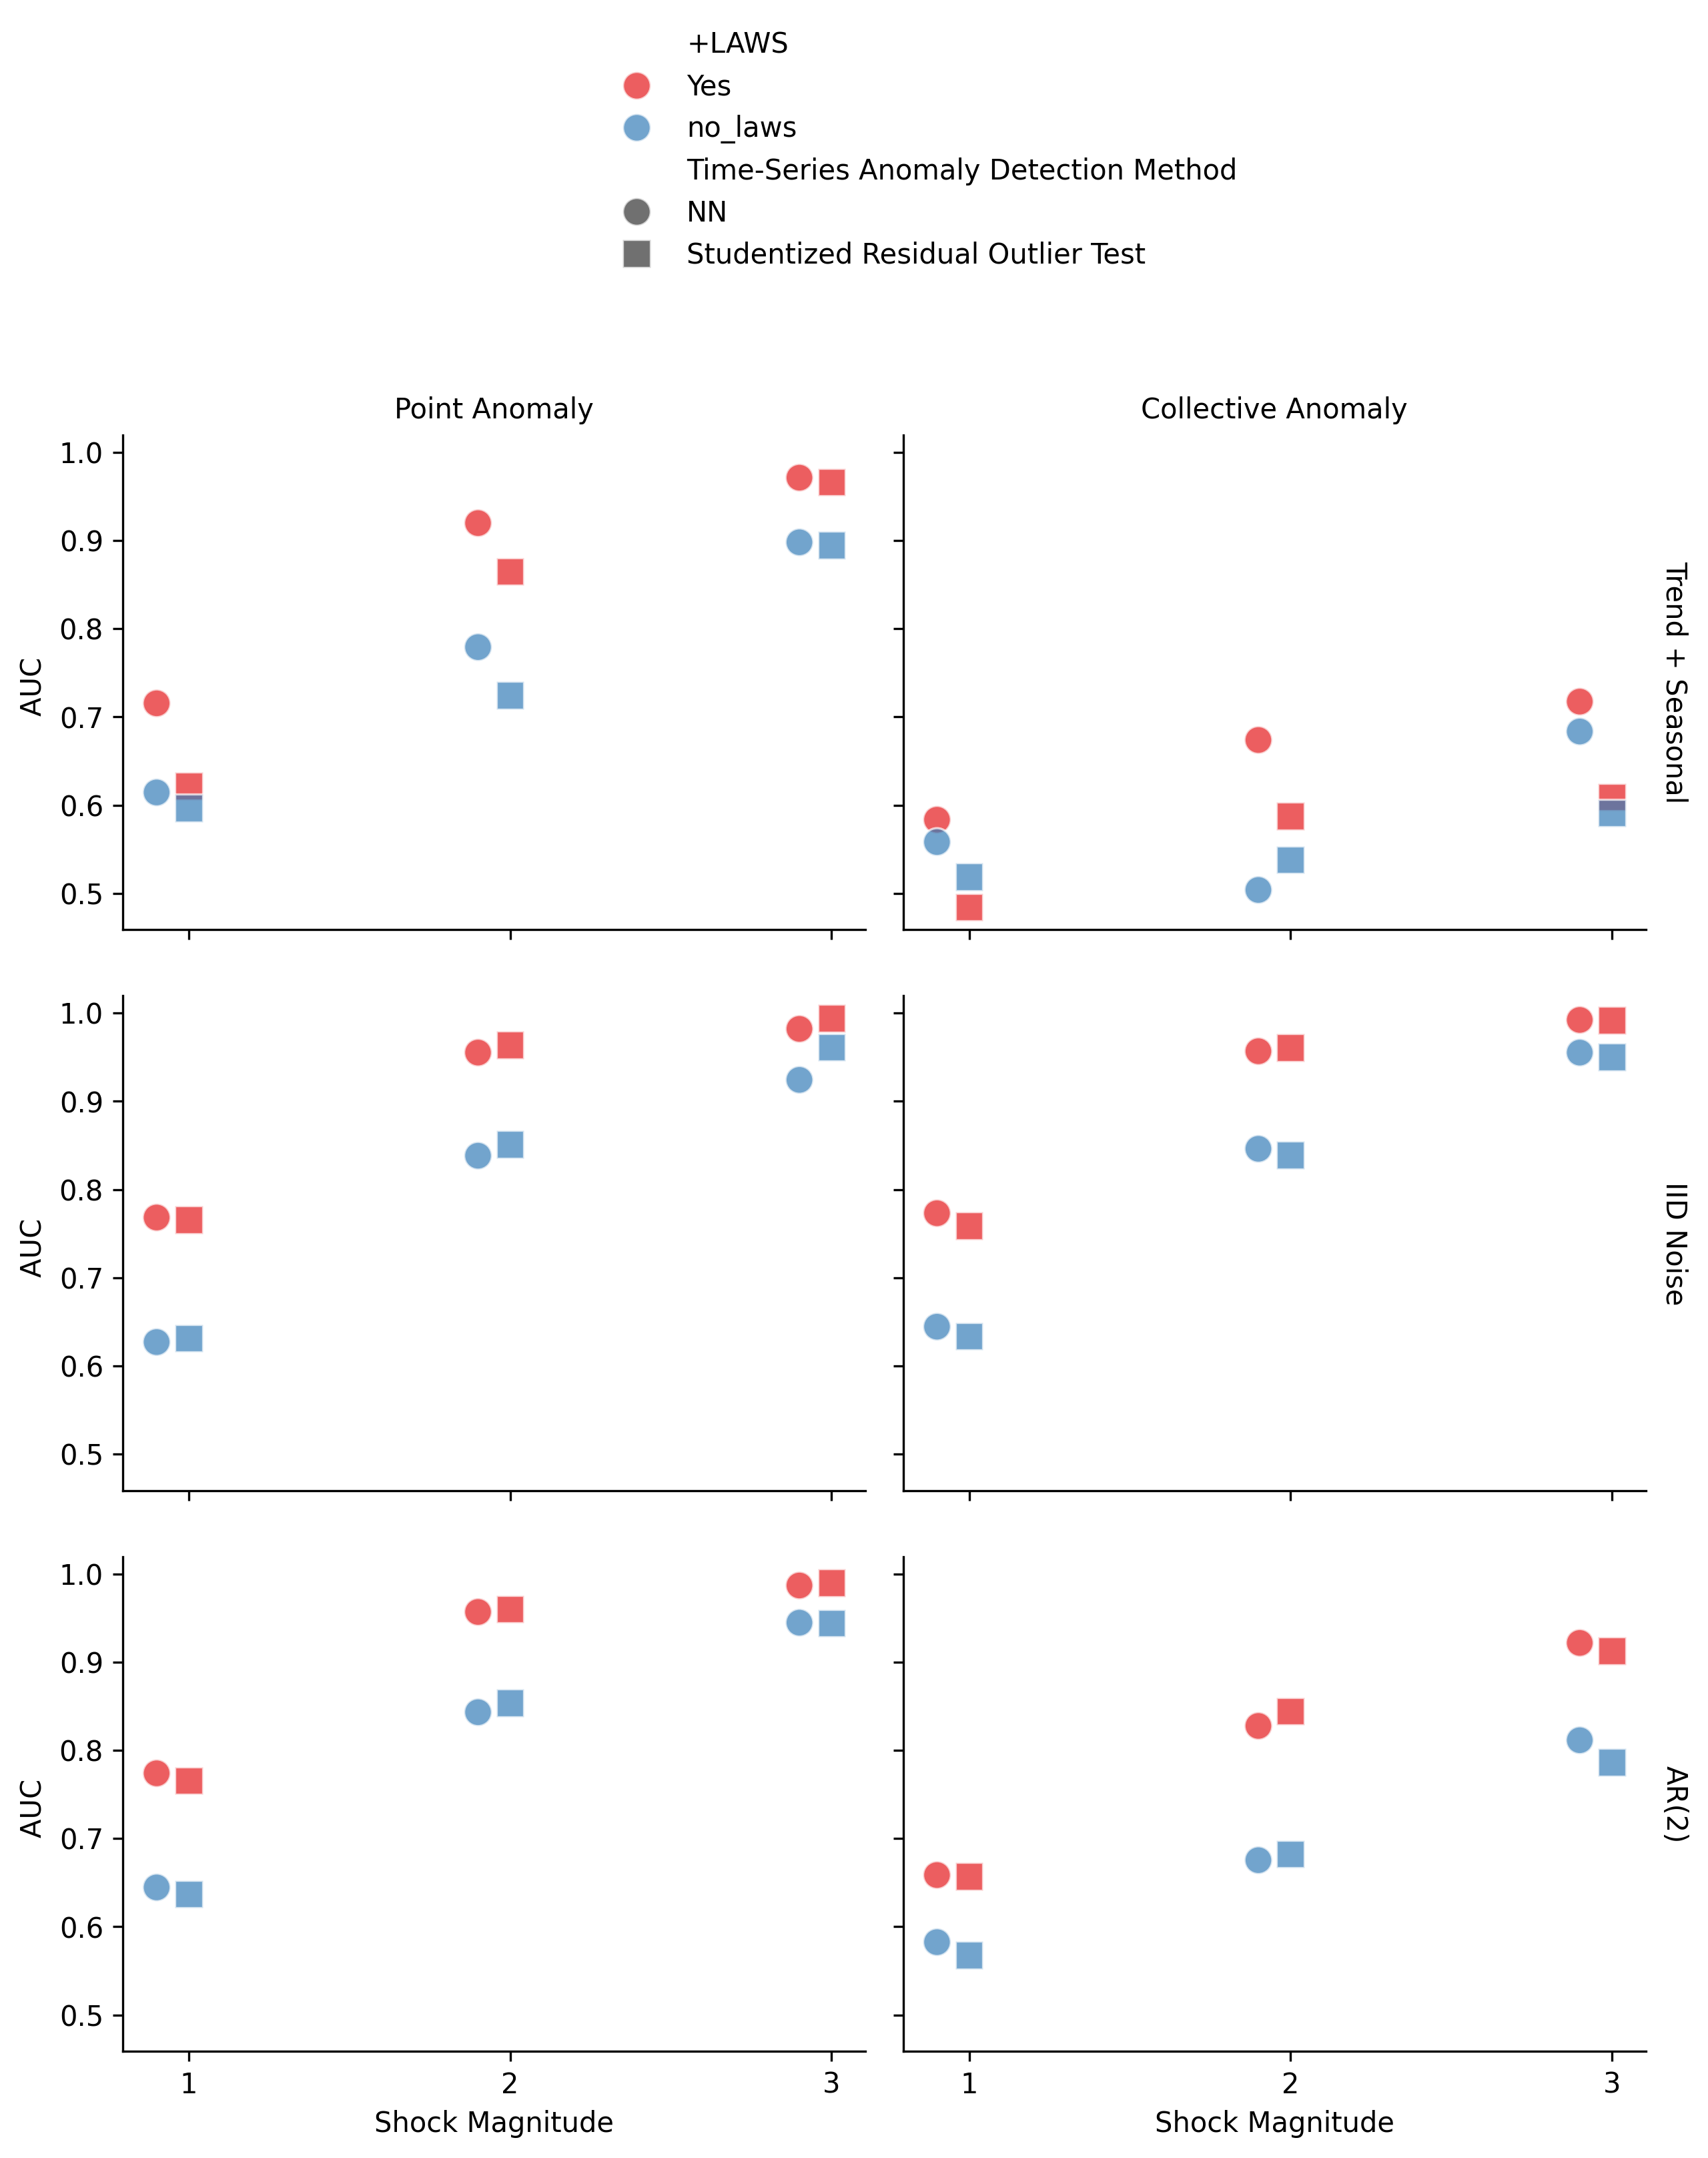
\includegraphics[width=\textwidth]{../figure/simulation_long_time_series.png}
    \caption{Long time series scenario. This figure assesses the performance of two time series anomaly detection methods: NN-based and Studentized Residual Outlier Test, under various conditions: trend and seasonal patterns, IID noise, and AR(2) processes. Both methods are evaluated for point and collective anomalies across shock magnitudes (1, 2, and 3), using the Area Under the Curve (AUC) metric. NN-based methods are depicted with circles, and Studentized Residual Outlier Test with squares. The presence of spatial anomaly detection by LAWS is indicated by green markers, while its absence is shown with red markers.}
    \label{fig: simulation long time series}
\end{figure}


\begin{figure}[h]
    \centering
    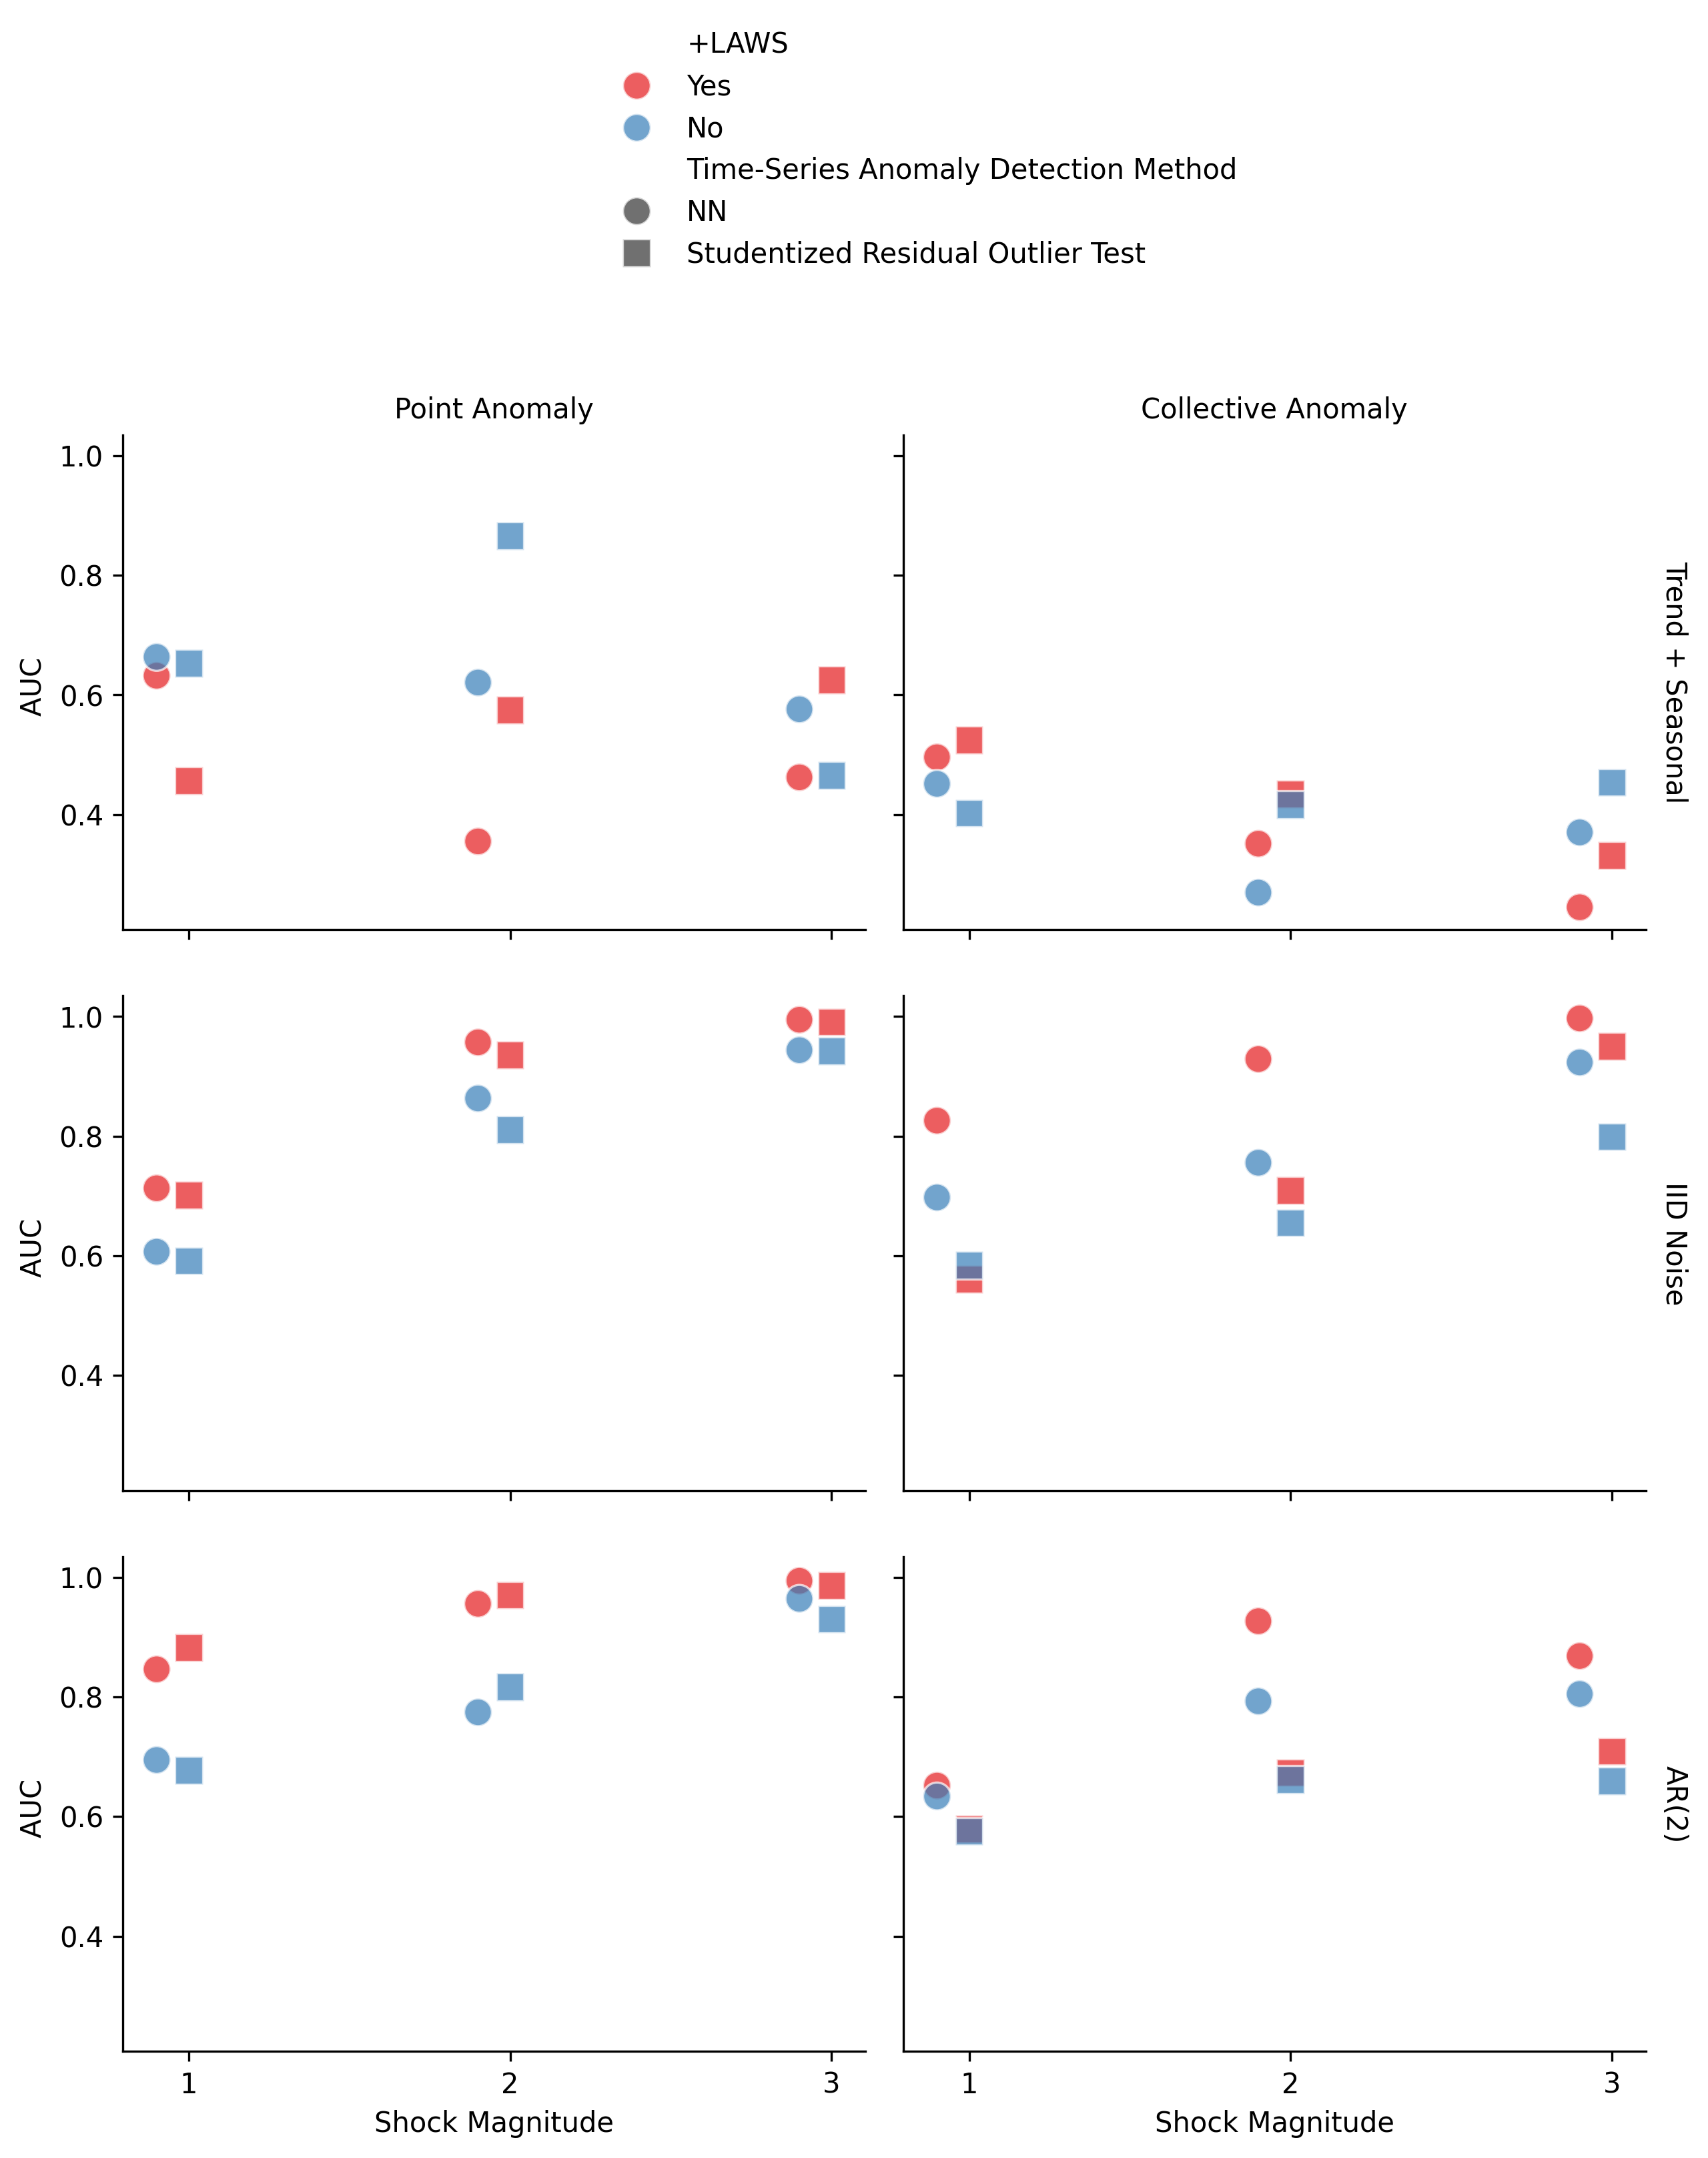
\includegraphics[width=\textwidth]{../figure/simulation_short_time_series.png}
    \caption{Short time series scenario. This figure assesses the performance of two time series anomaly detection methods: NN-based and Studentized Residual Outlier Test, under various conditions: trend and seasonal patterns, IID noise, and AR(2) processes. Both methods are evaluated for point and collective anomalies across shock magnitudes (1, 2, and 3), using the Area Under the Curve (AUC) metric. NN-based methods are depicted with circles, and Studentized Residual Outlier Test with squares. The presence of spatial anomaly detection by LAWS is indicated by green markers, while its absence is shown with red markers.}
    \label{fig: simulation short time series}
\end{figure}


%
%\subsection{Additional Simulation}
%The simulation conducted in the last section is general for We now conduct an additional simulation on a larger spatial grid and shorter time series, which is more similar to the real data we will be working on. For this simulation, we specifically focus on the algorithm's ability to detect different anomaly shapes and magnitudes. Let $\mathbb{D}_t = \{1, \ldots, 20\}$ and $\mathbb{D}_s = \{(x,y): x=1,\ldots,200, y=1,\ldots,200\}$. We define a subset $A \in \mathbb{D}_s \times \mathbb{D}_t$ as the location and time of potential anomalies. We set $\theta(s;t) = 1$ for $(s,t) \in A$ and $\theta(s;t) = 0$ for $(s,t) \in \mathbb{D}_s \times \mathbb{D}_t \setminus A$. We then generate $Y(s,t)$ using the following equation:
%\begin{equation}
%	Y(s;t) \sim [1-\theta(s;t)]\mathcal{N}(0, 1) + \theta(s;t)\mathcal{N}(\mu(s;t),1),
%\end{equation}
%where $\mu(s;t)$ represents the anomaly magnitude at location $s$ and time $t$.
%
%We consider various settings with different shapes of $A$ and anomaly magnitudes across space and time, as detailed in Table \ref{tab: configuration of anomaly}. Our two-step anomaly detection procedure is performed using the statistical method rather than the NN-based method for time series anomaly detection. The reasons are as follows: (1) There are 40,000 locations, which means training 40,000 individual models. This is impractical due to time constraints. (2) The time series consists of only 20 observations, which makes training with the NN-based method challenging. Additionally, as a forecasting-based method, the NN-based method requires historical data as input, meaning the first few steps cannot be identified as anomalies. Therefore, the statistical method is more appropriate for this scenario.
%
%We compare the standalone statistical method and the statistical method with the LAWS adjustment across all settings. Table \ref{tab: simulation_wildfire} shows the AUC scores for both methods across the four settings. The results demonstrate a significant improvement in anomaly detection accuracy with the LAWS adjustment, particularly when anomalies are spatially contiguous.
%
%




\section{Data Examples}\label{sec: real data analysis}
\subsection{Wildfire Detection}
The Sakha Republic, also known as Yakutia, is a vast region in the Russian Federation, characterized by its extreme climate. Wildfire detection in Sakha is of vital importance due to several factors. The region's vast forested areas, combined with its extreme climate, elevate the risk of wildfires, which can have devastating effects on the ecosystem and the local communities. Effective wildfire management and detection are crucial for minimizing damage and protecting lives and property. Our dataset spans from 2002 to 2021, with one image per year, each having dimensions of 278 by 229 pixels. These images represent the maximum Enhanced Vegetation Index (EVI) values observed during the peak growing season, as measured by the MODIS satellite system, see Figure \ref{fig: real data} Each pixel within an image, corresponding to a spatial resolution of 1km by 1km, captures the highest EVI reading for its respective location over the period from March 1st to September 30th of each year. Wildfires significantly reduce EVI values by causing vegetation loss and often affect large, interconnected areas. Our goal is to apply a two-step anomaly detection procedure to identify times and locations with unusually low EVI values, indicating the occurrence of wildfires in that year and locations.

\begin{figure}[h!]
    \centering
    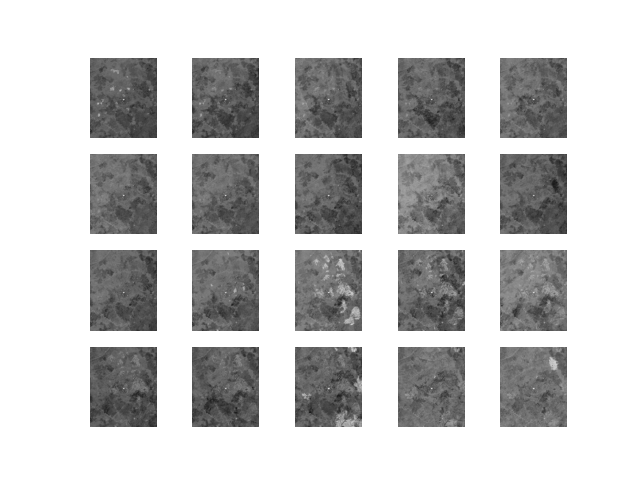
\includegraphics[width=\textwidth]{../figure/raw_data}
    \caption{Visualization of the raw max summertime EVI from 2002-2021. }
    \label{fig: real data}
\end{figure}



\subsection{Actual Data Example}
For the analysis of the real dataset, $\mathbb{D}_t=\{1, \ldots, 20\}$ and $\mathbb{D}_s=\{(x, y), 1 \leq x \leq 278, 1 \leq y \leq 229\}$. We apply both the NN-based and the statistical methods, with and without LAWS adjustment. Given the short time series, for the NN-based method, we set $H_{\mathrm{in}}=1$ and $H_{out}=1$ and train a single DLinear model for all locations. For all methods, we set the p-value threshold $\alpha=0.05$.

 It's important to note that we consider unusually low EVI values as indicative of potential fire events. Since the residual is the predicted value minus the actual value, unusually low EVI values result in unusually large residuals. Therefore, we only focus on large residuals. To accommodate this, we adjust the two-sided p-value used in Algorithm \ref{alg: convert errors to p-values} and Equation (\ref{eq: p-value}) to a one-sided p-value, defined as follows:
\begin{equation}\label{eq: one-sided p-value}
	p(s;t)= 1-\Phi_{L-5}\{Z(s;t)\}.
\end{equation}



The results for the NN-based method and the statistical method are shown in Figure \ref{fig: nn_real_data} and Figure \ref{fig: statistical_method_real_data}, respectively. The left panel in each figure shows fire detection by the standalone NN-based method, while the right panel includes the LAWS adjustment. In these figures, black areas represent detected ST anomalies, indicating wildfire occurrences.

The standalone versions of both methods show many scattered detections over the years. Since wildfires typically affect contiguous regions, these detections might be due to random errors. Additionally, both methods detected large areas of fire in 2013 and 2020, which, despite the lack of true fire occurrence data, seem dubious and might represent false alarms. With the LAWS adjustment, both methods prefer identifying contiguous regions as anomalies, aligning with the idea that wildfires affect continuous areas and demonstrating better robustness against noise compared to the standalone methods.



\begin{figure}[H]
     \centering
     
      \begin{subfigure}[b]{0.45\textwidth}
		\centering
		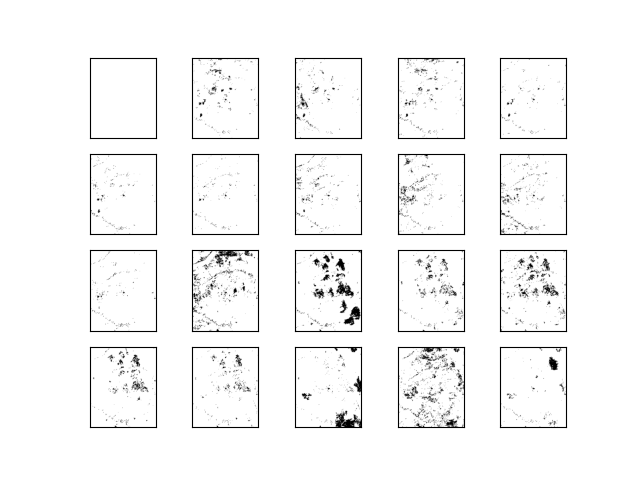
\includegraphics[width=\textwidth]{../figure/nn_no_laws.png}
		\caption{}
	 \end{subfigure}
         \hfill
      \begin{subfigure}[b]{0.45\textwidth}
         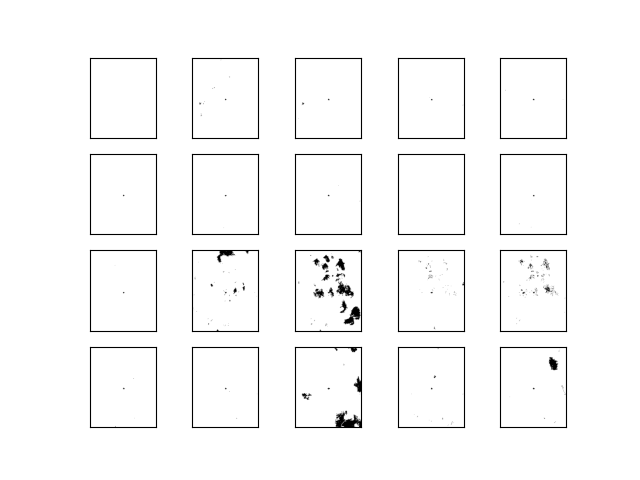
\includegraphics[width=\textwidth]{../figure/nn_laws.png}
         \caption{}
     \end{subfigure}
         \caption{Wildfire detection using the NN-based method. (a) Without LAWS adjustment, showing scattered detections that might include random errors. (b) With LAWS adjustment, focusing on contiguous regions, demonstrating improved robustness against noise and better alignment with the behavior of wildfires, which affect continuous areas. Black areas represent detected spatiotemporal anomalies, indicating potential wildfire occurrences.}
      \label{fig: nn_real_data}
\end{figure}



\begin{figure}[H]
     \centering
     
      \begin{subfigure}[b]{0.45\textwidth}
		\centering
		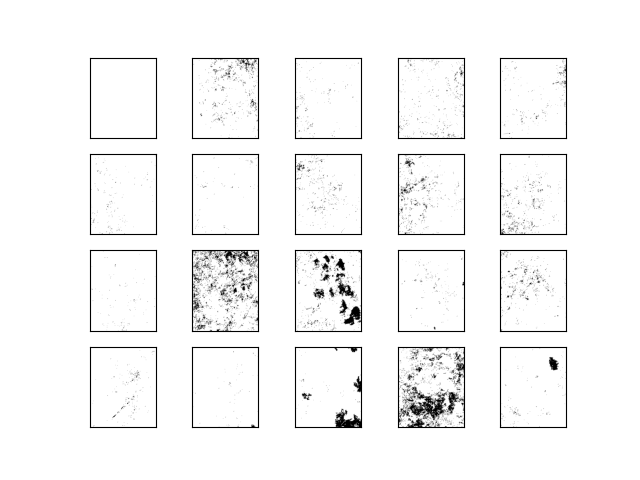
\includegraphics[width=\textwidth]{../figure/statistical_method_no_laws}
		\caption{}
	 \end{subfigure}
         \hfill
      \begin{subfigure}[b]{0.45\textwidth}
         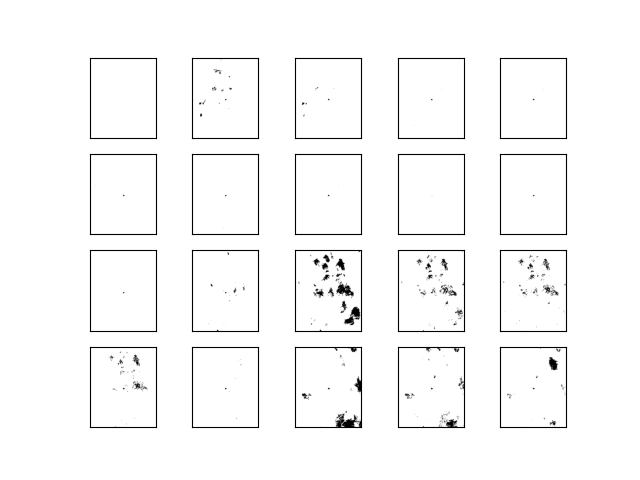
\includegraphics[width=\textwidth]{../figure/statistical_method_laws}
         \caption{}
     \end{subfigure}
         \caption{Wildfire detection using the statistical method. (a) Without LAWS adjustment, showing scattered detections that might include random errors. (b) With LAWS adjustment, focusing on contiguous regions, demonstrating improved robustness against noise and better alignment with the behavior of wildfires, which affect continuous areas. Black areas represent detected spatiotemporal anomalies, indicating potential wildfire occurrences.}
      \label{fig: statistical_method_real_data}
\end{figure}


%\begin{figure}[H]
%     \centering
%     
%      \begin{subfigure}[b]{0.45\textwidth}
%		\centering
%		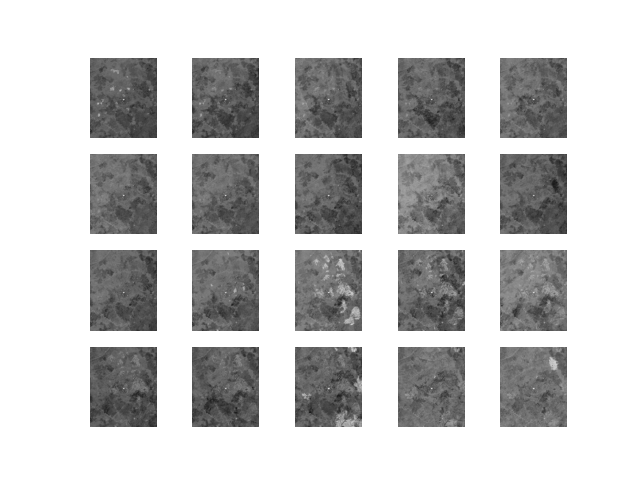
\includegraphics[width=\textwidth]{../figure/raw_data.png}
%		\caption{}
%	 \end{subfigure}
%         \hfill
%      \begin{subfigure}[b]{0.45\textwidth}
%         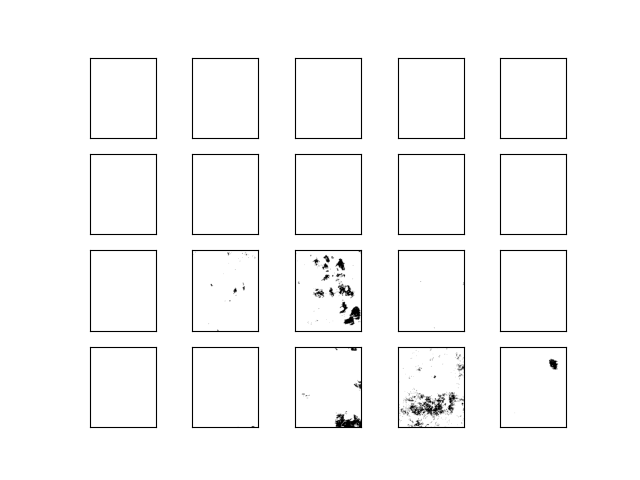
\includegraphics[width=\textwidth]{../figure/laws_0.05.png}
%         \caption{}
%     \end{subfigure}
%     \hfill
%      \begin{subfigure}[b]{0.45\textwidth}
%         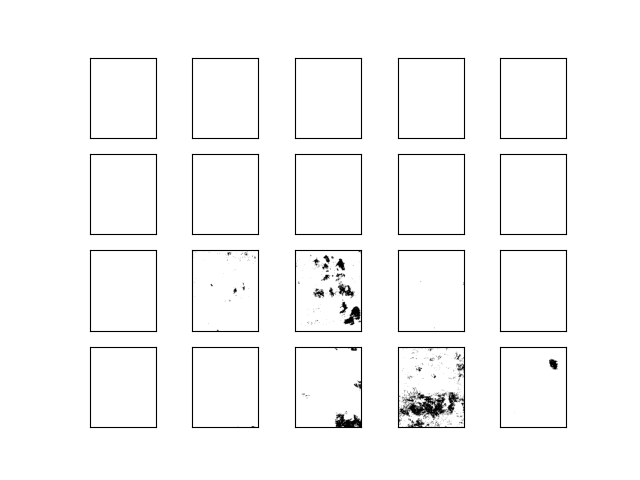
\includegraphics[width=\textwidth]{../figure/laws_0.1.png}
%         \caption{}
%      \end{subfigure}
%      \hfill
%       \begin{subfigure}[b]{0.45\textwidth}
%        \includegraphics[width=\textwidth]{../figure/laws_0.2.png}
%       \caption{}
%      \end{subfigure}
%     \caption{(a) Visualization of the raw max summertime EVI from 2002-2021. (b) Fire detection by standalone statistical time series anomaly detection method. (c) Fire detection by statistical method plus LAWS adjustment. Black-colored areas indicate detected wildfires within a specific year.}
%      \label{fig:real_data}
%\end{figure}

%
%\begin{figure}[H]
%     \centering
%     
%      \begin{subfigure}[b]{0.45\textwidth}
%		\centering
%		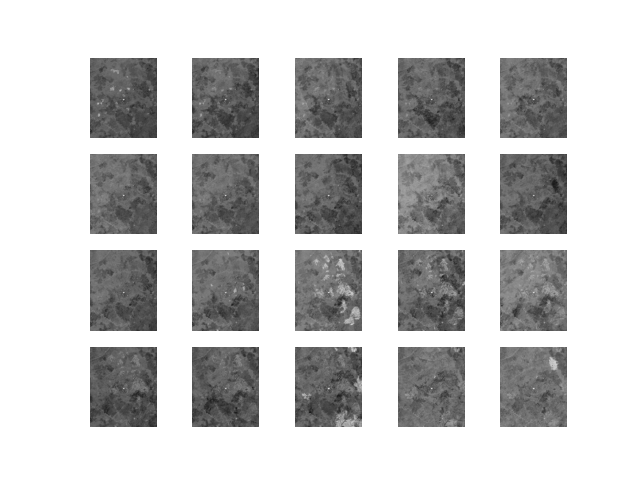
\includegraphics[width=\textwidth]{../figure/raw_data.png}
%		\caption{}
%	 \end{subfigure}
%         \hfill
%      \begin{subfigure}[b]{0.45\textwidth}
%         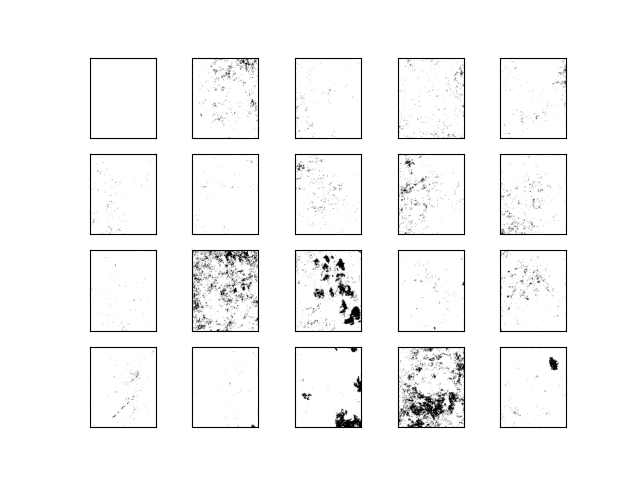
\includegraphics[width=\textwidth]{../figure/no_laws_0.05.png}
%         \caption{}
%     \end{subfigure}
%     \hfill
%      \begin{subfigure}[b]{0.45\textwidth}
%         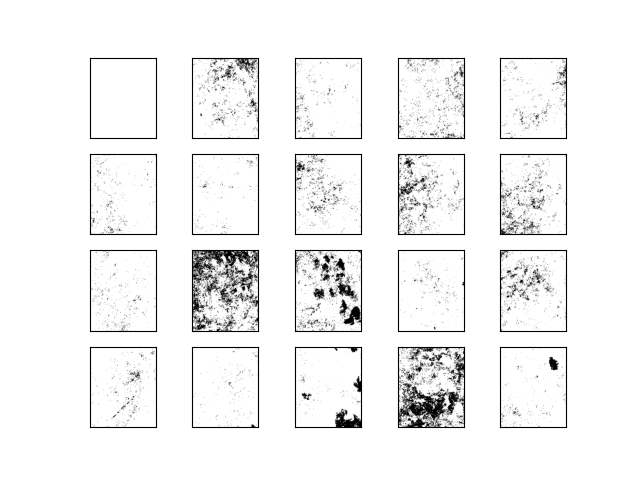
\includegraphics[width=\textwidth]{../figure/no_laws_0.1.png}
%         \caption{}
%      \end{subfigure}
%      \hfill
%       \begin{subfigure}[b]{0.45\textwidth}
%        \includegraphics[width=\textwidth]{../figure/no_laws_0.2.png}
%       \caption{}
%      \end{subfigure}
%     \caption{(a) Visualization of the raw max summertime EVI from 2002-2021. (b) Fire detection by standalone statistical time series anomaly detection method. (c) Fire detection by statistical method plus LAWS adjustment. Black-colored areas indicate detected wildfires within a specific year.}
%      \label{fig:real_data}
%\end{figure}
%




\section{Conclusion}
In this study, we develop an innovative two-step approach for spatiotemporal raster data anomaly detection. For time series anomaly detection, we present two methods: an NN-based method and a statistical method using studentized residuals. Through simulations, we show that the NN-based method is more accurate for anomaly detection than statistical methods when dealing with complex time series containing trends and seasonality due to its flexibility in learning from data. However, statistical methods remain robust alternatives when the time series is simple, and the number of observations is small. We also introduce the LAWS method to aggregate spatial information. The LAWS method was initially designed for spatial multiple testing. Through extensive simulations, we show that LAWS adjustment significantly improves the power of anomaly detection when anomalies are spatially contiguous, which is often the case for anomalies in spatiotemporal raster data. Finally, we apply the two-step anomaly detection method to wildfire detection, demonstrating the practical value of our research.


\bibliographystyle{apalike}
\bibliography{refs}


\clearpage

\appendix
\section{Commonly Used Time Series Models for Anomaly Detection}

\textit{Autoregressive Model (AR).} AR is a linear model where the current value $X(t)$ is based on a finite set of previous values of length $p$ and error terms $\epsilon(t)$. A common form AR$(p)$ model is:

\begin{equation}\label{eq:ar}
	X(t) = a_0 + \sum_{i=1}^{p}a_iX(t-i) + \epsilon(t).
\end{equation}
Here, the error values $\epsilon_t$ are assumed to be independent and identically distributed with mean 0 and variance $\sigma$. Denote $\hat{a}_0,\ldots, \hat{a}^p$ to be the least squared estimates of $a_0,\ldots, a_p$. Thus, the remainder,  at time $t$ is $R(t)=\hat{a}_0 + \sum_{i=1}^{p}\hat{a}_iX(t-i) - X(t)$.

\textit{Moving Average Model (MA).} The moving average model (MA) considers that the current observation $X(t)$ is a linear combination of the last $q$ prediction errors $\{\epsilon(t),\ldots,\epsilon(t-q)\}$. A common form of MA$(q)$ model is:
\begin{equation}
	X(t) = a_0+\sum_{i=1}^q a_i\epsilon(t-i)+\epsilon(t)
\end{equation}

\textit{Autoregressive Moving Average Model (ARMA).} ARMA model is the combination of AR and MA, and the basic form ARMA$(p,q)$ is:
\begin{equation}
	X(t) = \sum_{i=1}^{p}a_iX(t-i)+\sum_{i=1}^{q}b_i\epsilon(t-i)+\epsilon(t)
\end{equation}

\textit{ARIMA Model.} The ARIMA model is a generalization of the ARMA model and is often used when the time series data is non-stationary. In addition to the $p$ and $q$ parameters in the ARMA model, it also has a $d$ parameter which defines the number of times the time series is differenced. 

\textit{Simple Exponential Smoothing (SES).} Simple exponential smoothing uses a non-linear approach by taking the previous time-series data to predict, and assigning exponential weights to the observations:

\begin{equation}
	X(t+1)=\alpha X(t)+\alpha(1-\alpha)X(t-1)+\alpha(1-\alpha)^2X(t-2)+\ldots+\alpha(1-\alpha)^N X(t-N).
\end{equation}

%\textit{Collective and Point Anomalies (CAPA).} \citet{fisch2018linear} discussed a Collective and Point Anomalies (CAPA) algorithm focusing on collective anomalies detection. It assumes that the data $x_1,\ldots, x_n$ follow a parametric epidemic change-point model with a probability density function $f(x_t,\theta(t))$, and 
%
%
%\begin{equation}
%\theta(t)=
%\begin{cases}
%    \theta_1, s_1 < t < e_1 \\
%   
%    \cdots \\
%     \theta_K, s_K<t\leq e_K \\
%     \theta_0.
%\end{cases}
%\end{equation}
%Here, $\theta_0$ is the unknown parameter of the distribution for the normal data. $(s_1,e_1),\ldots, (s_K,e_K)$ are the $K$ anomalous segments when the model deviates from the normal behavior. Assume $e_1\leq s_2,\ldots,e_{K-1}\leq s_K$, the idea of CAPA is to infer the number, $\tilde{K}$, segment locations $(\tilde{s}_1, \tilde{e}_1), \ldots, (\tilde{s}_K,\tilde{e}_K)$ and $\tilde{\theta}_0$ to minimize the penalized cost function:
%\begin{equation}\label{eq:CAPA}
%	\sum_{t\notin [\tilde{s}_i+1, \tilde{e}_i]}C(x_t, \tilde{\theta}_0)+\sum_{j=1}^{\tilde{K}}\big[\min_{\tilde{\theta}_j}\{\sum_{t=\tilde{s}_j+1}^{\tilde{e}_j}C(x_t, \tilde{\theta}_j)\}+\beta],
%\end{equation}
%where $C(x, \theta)$ is chosen to be a negative likelihood function of $x$ under the parametric model with $\theta$. $\beta$ is commonly chosen to be $C\log(n)$, and the length of the segment $e_i-s_i$ is constrained to be greater than $l$. CAPA then minimizes the objective function (\ref{eq:CAPA}) using an optimal partitioning algorithm \citep{jackson2005algorithm}.
%
%\textit{Multivariate Collective And Point Anomalies (MVCAPA).} This algorithm is a multivariate version of CAPA. It assumes that the $p$ components of the time series are independent of one another in all aspects except the locations of collective anomalies, which can affect any subset of the components. (see \citet{fisch2021subset} for more details)

\section{Details of Kulldorff's Spatial Scan and Neil's Fast Subset Scan}
\textit{Kulldorff's Spatial Scan.}
The scan statistic was originally presented by \citet{naus1965distribution} to address the multiple testing problem. However, it is restricted to finding a fixed-size anomalous region. \citet{kulldorff1995spatial} proposed a spatial scan statistic, which extends the original scan statistic to detect variable size regions. In Kulldorff's formulation, we have a count $c_i$ and a population $p_i$ at each location $s_i$, and each count $c_i$ follows a Poisson distribution with mean $q_ip_i$, where $q_i$ is the unknown risk. Then, the spatial scan statistic tries to detect spatial regions where $q_i$ are significantly higher (or lower) inside the region than that outside the region. More precisely,  the null hypothesis $H_0$ is $c_i\sim \mbox{Poisson}(q_{0}p_i)$ for all locations $s_i$, and the alternative hypothesis $H_1(S)$ is that there exists a region $S$, where $c_i\sim \mbox{Poisson}(q_{in}p_i)$ for all locations $s_i$ in $S$, and $c_i\in \mbox{Poisson}(q_{out}p_i)$ for all locations $s_i$ outside $S$.  The likelihood ratio test for any region $S$ is 
\begin{equation}
	F(S)=
\begin{cases}
    (\frac{C_{in}}{P_{in}})^{C_{in}}(\frac{C_{out}}{P_{out}})^{C_{out}}(\frac{(C_{in}+C_{out})}{(P_{in}+P_{out})})^{-(C_{in}+C_{out})}, \mbox{if } \frac{C_{in}}{P_{in}}>\frac{C_{out}}{P_{out}}, \\
    1, \mbox{if }\frac{C_{in}}{P_{in}}\leq \frac{C_{out}}{P_{out}}.
\end{cases}
\end{equation}
Notice that, $q_{0}$, $q_{in}$, and $q_{out}$ are substituted by their maximum likelihood estimates in the above equation. $C_{in}$ and $C_{out}$ represent the aggregate count $\sum c_i$ inside and outside region $S$, respectively. \citet{kulldorff1997spatial} also proved that this likelihood ratio statistic is more likely to detect the anomaly than any other test statistic under a fixed alarm rate and a given set of regions searched. Based on the test statistic $F(S)$, we can search for the region $S^*$ that achieves the highest score $F(S^*)$. However, searching for the highest score region requires a large number of searches and evaluations, which makes it computationally infeasible. Therefore, in practice, we typically restrict our search to a given shape region with varying sizes. The region $S^*$ which has the highest score among all regions $S$ that have been evaluated is considered the most anomalous region. To obtain its statistical significance (p-value), we use a technique called Monte Carlo randomization \citep{dwass1957modified}. The intuition is to generate a reference distribution for $F(S^*)$ using a bunch of permuted replication of the original data (see \citet{kulldorff2005space} for more details).

\textit{Fast Subset Scan.}
Kulldorff's spatial scan statistic is in general a powerful method for spatial anomaly detection, but it has two main limitations. First, the spatial scan requires us to search over a huge set of regions to find the most anomalous one. This is very computationally intensive in practice when the spatial dataset contains thousands or even millions of locations. If we only search a given shape of regions, the computation would be sped up but the power of finding the true anomaly would be largely decreased. Second, there are only two statistical models (Poisson and binomial) in Kulldorff's spatial scan approach, which greatly limits the application domain. To make the spatial scan approach scalable, \citet{neill2012fast} proposed a fast subset scan statistic, which significantly reduces the search time by only searching a small fraction of regions and proving that the other regions do not need to be searched. The fast scan approach treats anomaly detection as a search over subsets of data and finds the subset which maximizes some score function. It proves that many commonly used functions such as Kulldorff's spatial scan statistic satisfy a property called ``linear time subset scanning" (LTSS) and this property enables us to find the highest-scoring unconstrained subset by evaluating only $N$ of the $2^N$ possible subsets. However, an unconstrained search over subsets can return dispersed sets of locations that we would not consider to be ``spatial anomaly". To incorporate spatial information in the LTSS framework, \citet{neill2012fast} also proposed two proximity-constrained subset scan methods: fast localized scan and fast localized multiscan. The fast localized scan considers each spatial location $s_i$ as a possible center of the region, then define its local neighborhood $S_i$ using ``$K$-nearest neighbors" or ``fixed radius" approach, and finally, uses LTSS to efficiently maximize over all subsets $S\subseteq S_i$. The disadvantage of the fast localized scan is that it enforces a hard constraint on the maximum size of the anomalous region, which is often unknown in real data. In addition, when the neighborhood is large, it is still possible to obtain dispersed subsets that look less likely to be true ``spatial anomalies". The other fast localized multiscan approach attempts to find the trade-off between score and size by computing the highest scoring subset for each neighborhood size $k=1,\ldots, N$. However, it is too computationally intensive in practice. 

Based on fast subset scan and the LTSS framework,\citet{speakman2016penalized} proposed a ``Penalized Fast Subset Scanning (PFSS)" approach, which enables ``soft constraints" instead of hard constraints on spatial proximity. PFSS with soft proximity constraints allows us to take additional spatial information into account, rewarding spatial compactness and penalizing sparse regions within a local neighborhood.








\end{document}

